\documentclass{article}
\usepackage{graphicx} % Required for inserting images
\usepackage{natbib}
\usepackage{float}    % Required for fixing the position of the figure

\title{\textbf{Project Report}\\ Grain Analysis Using Computational Methods}
\author{Zulkuf Azizoglu, Cinar Turhan, Fehmi Ozbayrak}
\date{October 2024}

\begin{document}

\maketitle

\section*{Executive Summary}
This project aims to investigate image processing methodologies and calculations to extract grain and rock properties from rock images. We seek to create an established software pipeline that allows the end user to confidently input the desired image and receive grain and rock properties as output in a streamlined, non-intervening way. Additionally, the project contributes to the open-source community in the field of geoscience.

\section{Introduction}
Grain properties such as sphericity, roundness, and size distribution are crucial for geoscientists as they provide insights into sediment transport, depositional environments, and the physical and chemical processes that shape geological formations \citep{blott2006}. Many different attempts have been made to define these properties, and obtain them either by manual methods or algorithmic approaches \citep{cox1927method, krumbein1941measurement, wadell1932volume, zheng2015traditional}. Consequently, there is not an agreement between definitions of these properties and ways to calculate them. In addition, a notable portion of the existing methodologies are not well-documented with a suitable test case that introduces replicability; making the methodologies hard-to-reach for many geoscientists. Also, with the recent development of image processing and statistical methods, there is a significant opportunity to apply these methodologies to geoscientific settings to tackle these long-standing challenges. Advanced image processing techniques, such as machine learning algorithms and morphological analyses, can automate the extraction of grain properties from images, thereby reducing subjectivity and improving accuracy \citep{karpatne2018machine, peregrina2013automatic, williams1998sand, arasan2011effect}. By leveraging these technologies, we can explore the true characteristics of the relationship between the physical phenomena and the grain properties, and create reliable models that geoscientists can use to validate their own data through comparison, ultimately contributing to a more unified approach in the study of grain properties and their geological implications.

In this work, we try and evaluate the existing image processing and computational techniques to determine grain properties in a given rock image; and we streamline our findings in a user-friendly open-source software. The software is capable of extracting several grain properties estimated by the methodologies given by the previous work, and it is scalable to a larger software with the addition of new methods. In Section~\ref{Sec: Work}, we give an overview of our pipeline and the explanation of the individual parts of the workflow. In Section~\ref{Sec: Results}, we report and explain our findings. In Section~\ref{Sec: Conclusion and Future Work}, we summarize our work and define the next steps for this project.
\section{Work}{\label{Sec: Work}}

The summary of the workflow can be given as the following flow chart:

\begin{figure}[H]
    \centering
    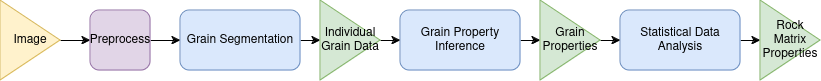
\includegraphics[width=\textwidth]{workflow_diagram.png}
    \caption{Flow chart of the workflow. The yellow container represents the input, which is the image file. Blue containers represent the main steps of the workflow, while the purple container denotes the optional preprocessing step. Green containers indicate the outputs of the process.}
    \label{fig:workflow_diagram}
\end{figure}

\subsection{Image}
Here, the image is any given 2D rock matrix image. There is no scale distinction as the methodologies aim to determine the grain properties regardless of the scale. We will use the image taken from Coconino, Arizona.

\begin{figure}[H]
    \centering
    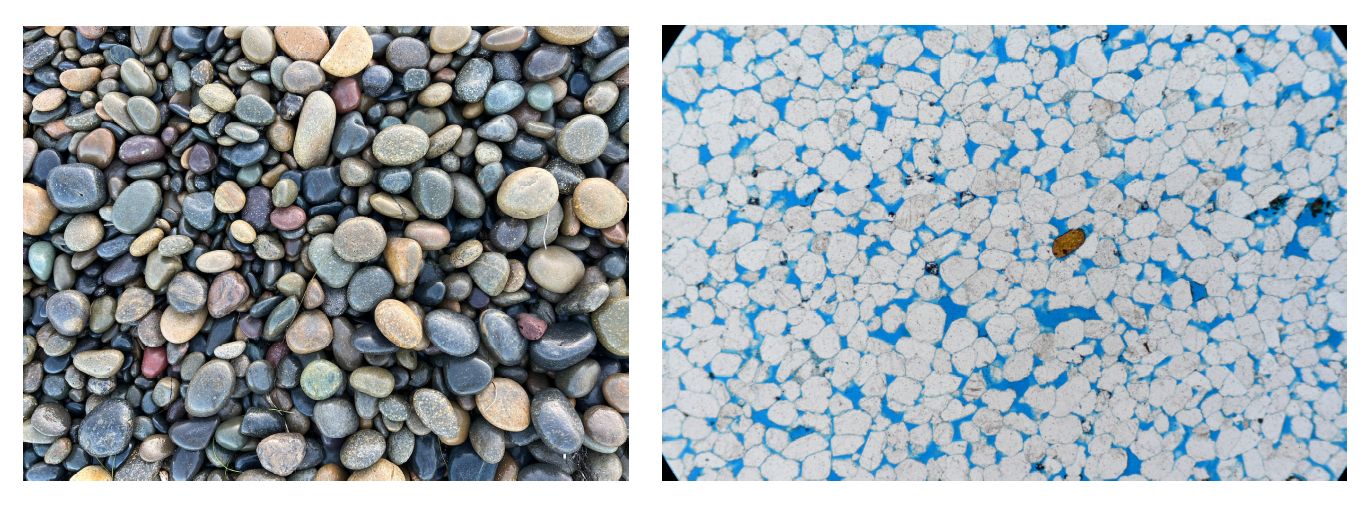
\includegraphics[width=\textwidth]{rock_samples.png}
    \caption{Possible images for the workflow. Since the idea is the same, both of these images can be used with this workflow despite the difference in scale.}
    \label{fig:rock_samples}
\end{figure}

\subsection{Preprocess}
Zulkuf sende (ilastikten falan bahsedersin)

\subsection{Grain Segmentation}
For grain segmentation, we use 'Segmenteverygrain' Python package \citep{zsylvester_segmenteverygrain_2023}. This package is designed to detect grains or grain-like objects in images, providing a valuable tool for determining grain size and shape, tasks that are common in geomorphology and sedimentary geology. 'Segmenteverygrain' leverages the Segment Anything Model (SAM), developed by Meta, to obtain high-quality outlines of grains \citep{kirillov2023segany}. However, SAM requires prompts for every object it detects, and when operated in 'everything' mode, it tends to be slow and may produce many overlapping masks, along with non-grain objects from the background. To mitigate these issues, 'Segmenteverygrain' incorporates a Unet-style, patch-based convolutional neural network, which performs an initial segmentation to generate prompts for SAM. Although this approach may miss some grains, the segmentations it produces are generally of high quality.

\subsection{Individual Grain Data}
"Segmenteverygrain" is able to calculate some important individual grain data, such as the shape of the grain as a polygon with the correct centroid coordinate, area of the shape, major and minor axis lengths and major and minor axis directions.

\subsection{Grain Property Inference}
We investigate several approaches for infering different grain properties.
\subsubsection{Sphericity}
Given by \citet{zheng2015traditional}, Area Sphericity ($S_{A}$) are calculated as follows:
$$S_{A}=\frac{A_{S}}{A_{cir}}$$
where $A_{S}$ is the area of the grain, and $A_{cir}$ is the area of circle that has the radius equal to major axis length, $L_{major}$
and Width-to-length Ratio Sphericity is calculated as:
$$S_{WL}=\frac{L_{minor}}{L_{major}}$$
where $L_{minor}$ and $L_{major}$ are minor and major axis lengths, respectively.
\citet{wadell1932volume} ... Zulkuf sende
\subsubsection{Sortedness}
... Zulkuf sende
\subsubsection{Roundness}
Different attempts have been made for roundness, such as:
- Unwrapping the curve to polar coordinates using distance from centroid, then performing Fast-Fourier Transform (FFT) on the curve
- Calculating fractal dimension for the unwrapped curve as a measure of roughness
- Tracing the curve for derivatives and trying to investigate the derivative distributions
- Trying to investigate the differences between the curve and its convex hull
\subsection{Results}
\begin{figure}[H]
    \centering
    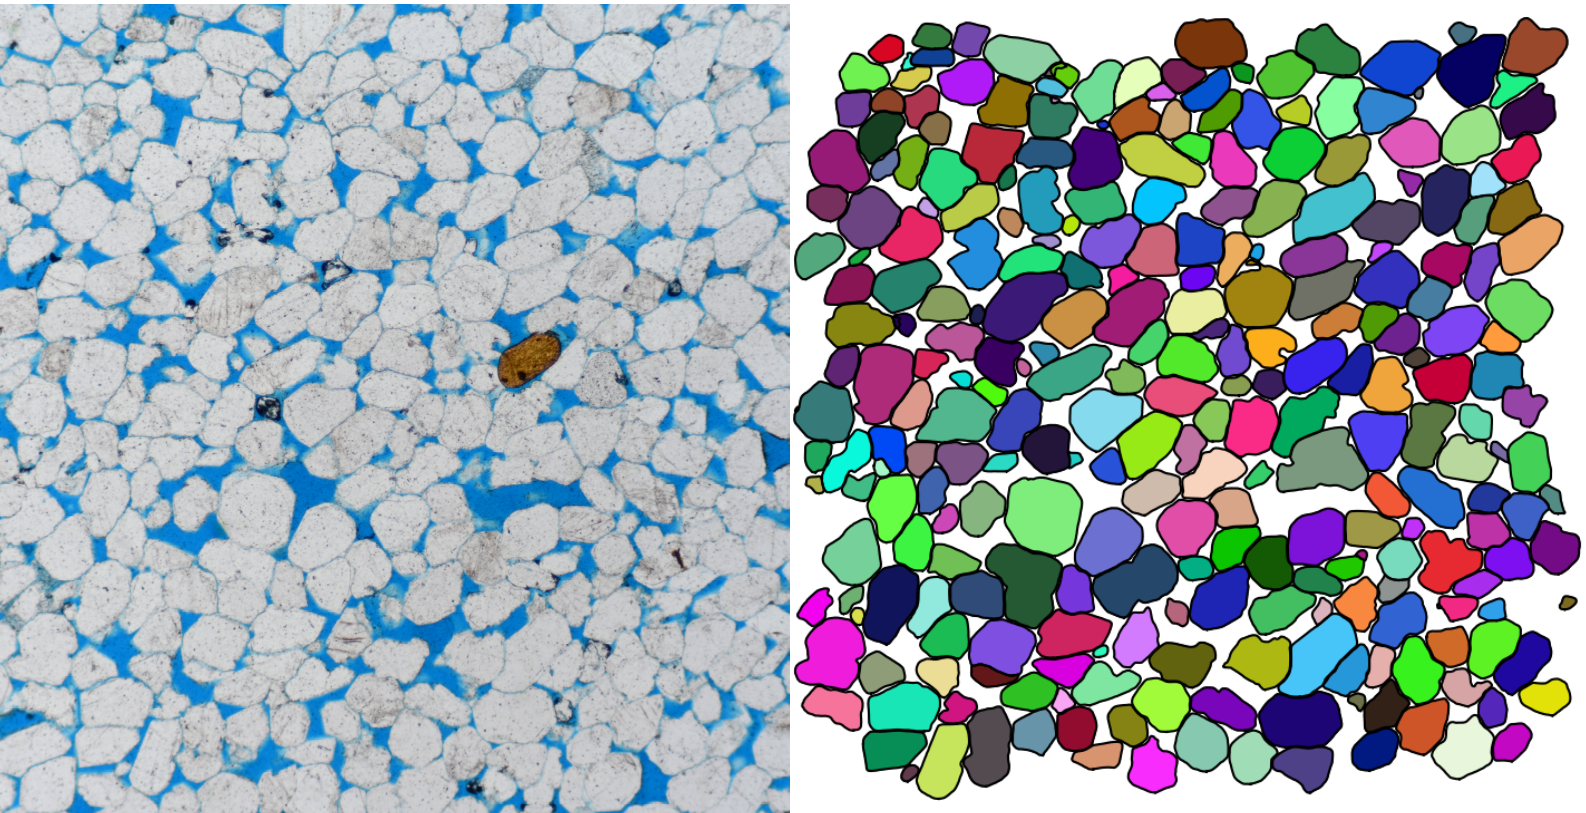
\includegraphics[width=\textwidth]{coconino_segmented.png}
    \caption{Output of the Coconino sample image (left) and the segmented image (right). Grains are colored differently to ensure visibility.}
    \label{fig:coconino_segmented}
\end{figure}

Results from segmentation indicate that 'Segmenteverygrain' algorithm works properly.

\begin{figure}[H]
    \centering
    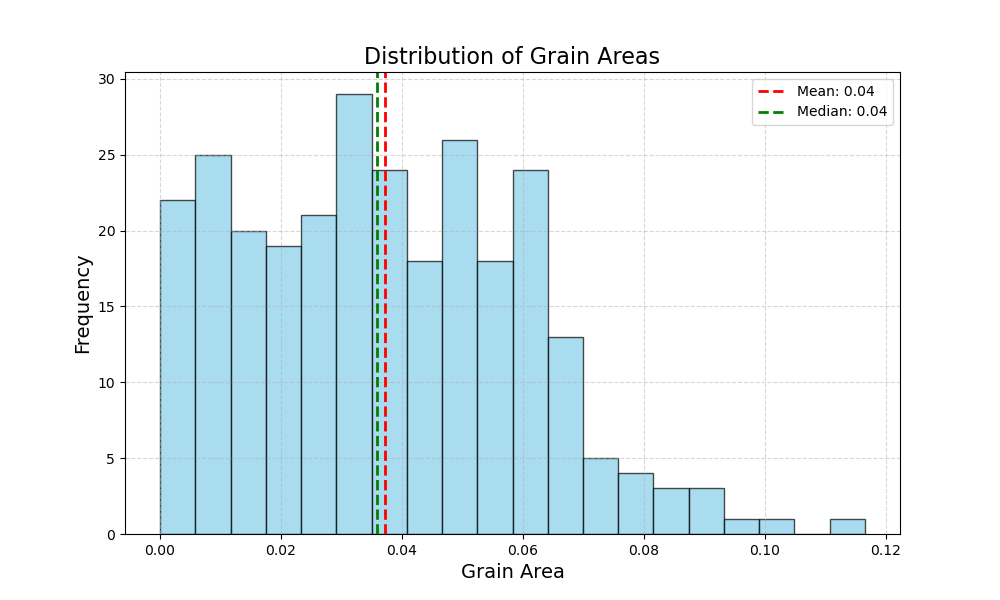
\includegraphics[width=\textwidth]{area_histogram.png}
    \caption{Histogram of grain areas.}
    \label{fig:area_histogram}
\end{figure}

The workflow is able to obtain the histogram of grain areas. One important note here is that the adjustments in the segmentation part must be made for the variables that determine the scale of the image (n\_points and units\_per\_pixel)

\begin{figure}[H]
    \centering
    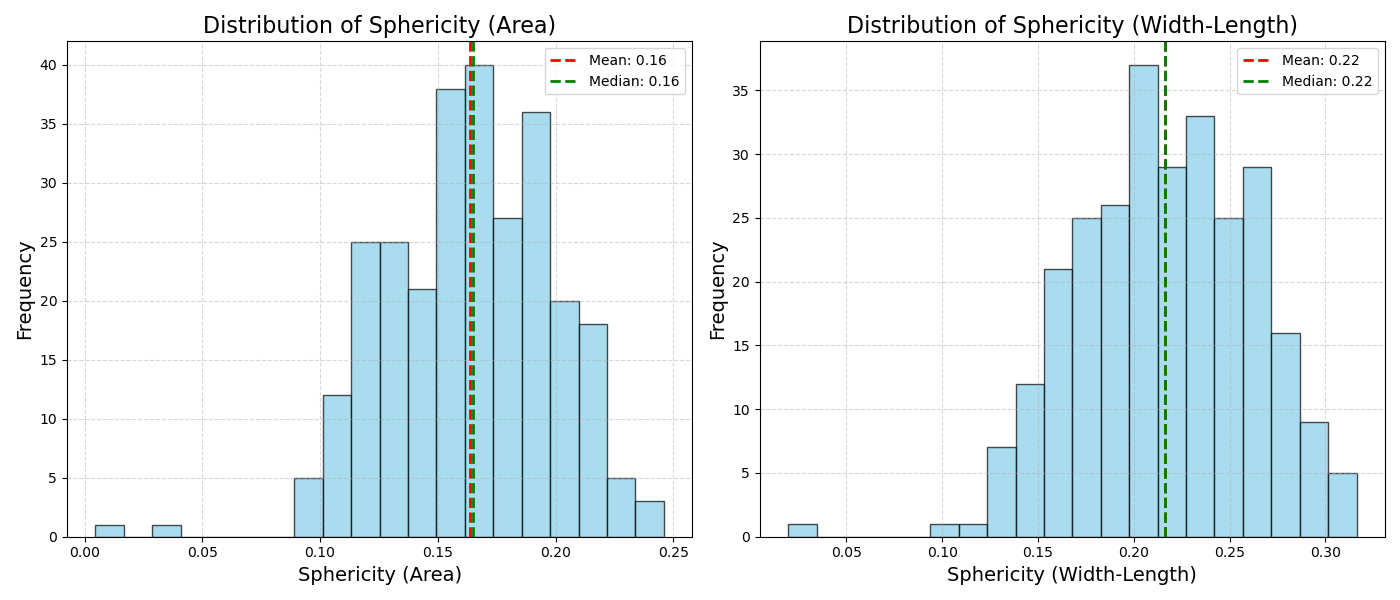
\includegraphics[width=\textwidth]{sphericity_histogram.png}
    \caption{Histogram of sphericity.}
    \label{fig:sphericity_histogram}
\end{figure}

The distributions for Area Sphericity and Width-to-lenth Ratio Sphericity seem quite reasonable, and they agree with each other, both having mean values around $0.16-0.22$.

--Zulkuf sende

-- Sortedness de sende

For roundedness, we have attempted several methods to reveal a relationship between the curve and the grain properties.

\begin{figure}[H]
    \centering
    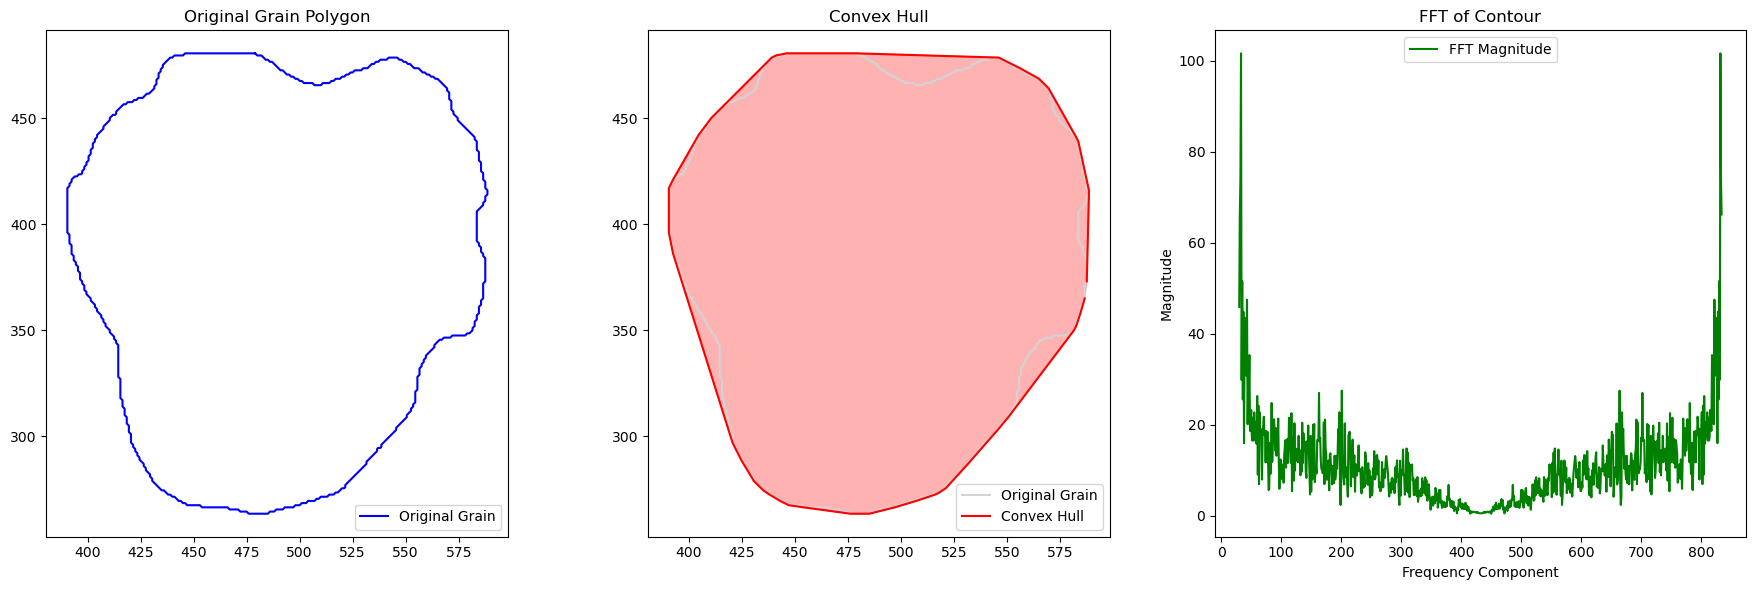
\includegraphics[width=\textwidth]{convex_hull_fft.png}
    \caption{Convex hull and FFT curves for a tested grain.}
    \label{fig:convex_hull_fft}
\end{figure}
\begin{figure}[H]
    \centering
    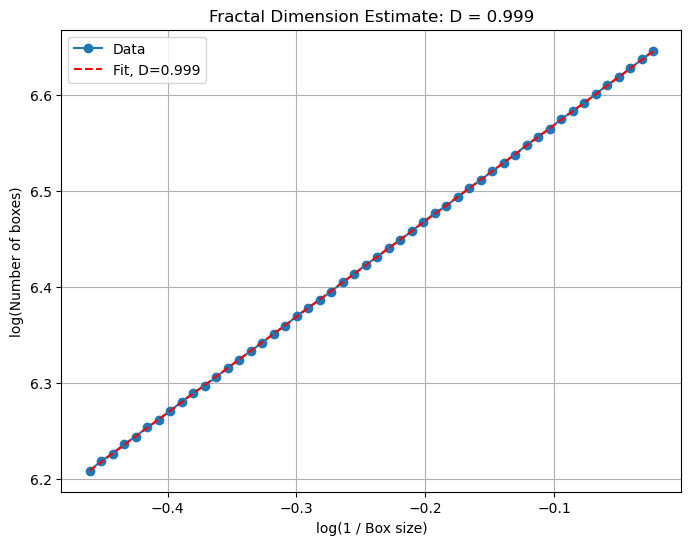
\includegraphics[width=\textwidth]{fractal.png}
    \caption{Box-counting fractal dimension for the tested grain.}
    \label{fig:fractal}
\end{figure}
\begin{figure}[H]
    \centering
    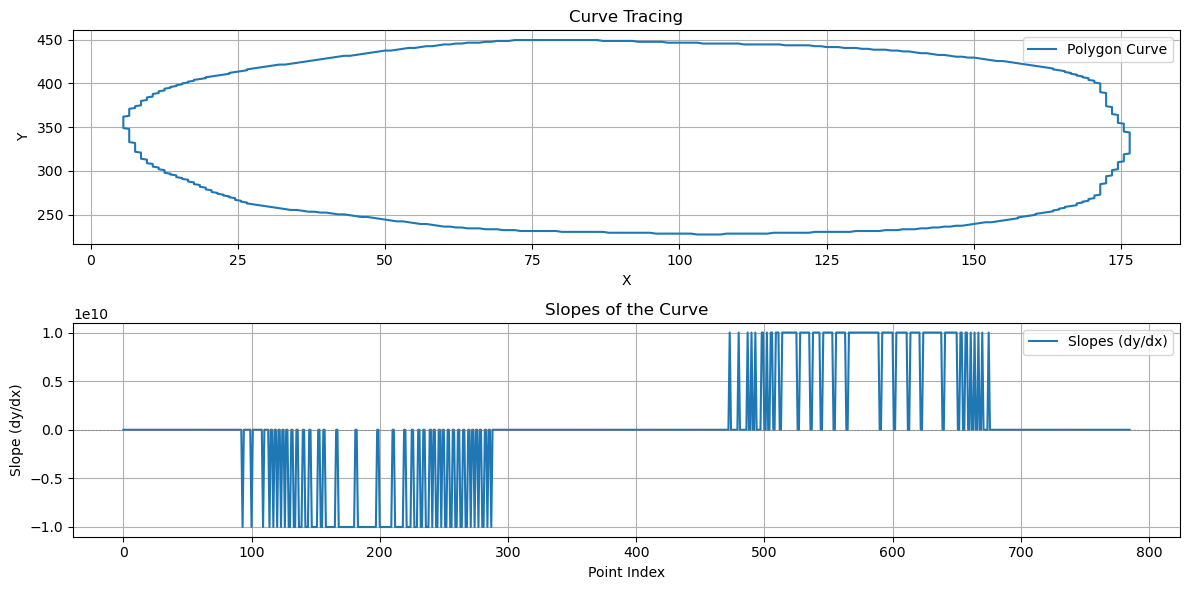
\includegraphics[width=\textwidth]{derivative_tracing.png}
    \caption{Derivative of the curve trace. The curve is traced started from an arbitrary point. In every increment, we calculated the derivative and investigated the distribution of the derivatives at the end.}
    \label{fig:derivative_tracing}
\end{figure}

We investigated FFT and Box-counting Fractal Dimension for possibly identifying the relatively high-frequency component of the roughness. However, interestingly, although we have the polygon for each grain, the resulting contours suffered from the low resolution in these analyses. In addition, no distinction was observed between the tried samples of different roundedness. Similarly, convex hull also had no explicitly notable correlation with roundedness. Derivative tracing, on the other hand, showed a bit sensitivity to roundedness, as more angular grains had oscillations in slope (y-axis) closer to the middle point index, however, there was no obvious way of mapping that to a roundedness metric value, and there were simply too many exceptional case that didn't follow this pattern.

\section{Conclusion \& Future Work}
In this work, we have attempted to build a workflow pipeline that would yield grain and rock properties with an image input. Some of the methods we tried were successful and some of them were not useful, or needed more detailed work. The greatest challenge associated with the project was the lack of labeled data. Given that such a labeled data would exist, a preliminary neural network model (a CNN, for instance) could have been built to provide the sphericity and roundedness values. This model then would also be used for understanding the physical phenomena and finding more direct and explicit correlations between the grain morphology and the grain properties. This is why, the greatest value lies in the creation of such a labeled data and making it open-source, and also completing the given workflow with other computational methods of calculating the grain properties to make it a full-fledged software.




\bibliographystyle{plainnat}
\bibliography{refs} % This assumes your BibTeX file is named 'refs.bib'.
\end{document}
